\chapter{Deseño e implementación de BikeCam}
\label{chap:implementacion_dispositivo}
\lettrine{N}{este} capítulo afondarase no desenvolvemento do dispositivo comezando polo aspecto físico profundando na construción do dispositivo e a implementación do sofware tendo en conta os problemas xurdidos e as solucións aplicadas.

\section{Estrutura xeral de BikeCam}
O dispositivo BikeCam componse de catro módulos principais. Son os seguintes.
\begin{itemize}
  \item Rasberry Pi Zero

    É o módulo principal sobre o que se apoiaran o resto. A súas funcións principais son as do procesamento, as comunicacións e o control do resto de módulos. Depende dunha alimentación de 5V para funcionar.
  \item LEDs

    Este módulo componse como mínimo dunha ou vairas series LEDs RGB direcionables. Para funcionar necesita alimentación a 5V é unha liña de datos conecta a Rasberry Pi, pode requirir un conversor lóxico de nivel nesta conexión.
  \item Cámara

    Este módulo se conecta directamente a Rasberry Pi, da que recibe alimentación e control e devolve o vídeo capturado.

  \item Alimentación

    Este módulo pode implementarse de duas maneiras.
    \begin{itemize}
      \item Unha batería USB que alimenta a Raspberry Pi, e esta a súa vez os LEDs e a cámara.
      \item O módulo LipoPi, encargado da alimentación enerxética do dispositivo na versión con batería interna. Conta cunha chip de alimentación Adafruit Powerboost 1000C un pulsador e unha serie de resistencias díodos e condensadores xunto cunha batería de 3.7V. Proporciona alimentación a Rasberry Pi e os LEDs, utiliza unha conexión coa Rasperry para informar do estado da batería, outro pin para informar a Raspberry do premido do pulsador e unha ultima liña de conexión coa que a Raspberry mantén o chip aceso.
    \end{itemize}
\end{itemize}

\section{LEDs}

Crearanse dous prototipos con dúas configuracións de LEDs diferentes, ambas contarán cun anel de 8 LEDs \emph{RGB} direccionables WS2812B, que conta cun tamaño perfecto para colocar arredor da cámara, a segunda opción contara ademais con dúas tiras de 8 LEDs cada unha que se utilizaran como indicadores de xiro para aumentar a visibilidade.
\subsection{Conexión coa Raspberry Pi}
Estes LEDs contan con catro puntos de conexión entrada de voltaxe, terra, entrada de datos é saída de datos.

A voltaxe necesaria para alimentalos e de 5V, aínda que na maioría dos caso o fabricante indica un soporte a voltaxes de entrada de entre 4V e 7V. A Raspberry Pi conta con pins de saída a 5V conectada directamente a entrada, sen contar coa limitación dun fusible como noutras versións da placa, polo que pode alimentar os LEDs directamente pero xa que cada LED pode chegar a consumir ata 60mA e os pins de 5V da Raspberry poden proporcionar ata 300mA~\cite{molloyRaspberryPiFondo2018} e facer pasar polo \emph{power rail} unha corrente excesiva podería provocar danos ou unha aumento da temperatura da placa implicando menor velocidade e maior consumo. Tendo en conta que o fabricante non recomenda que a placa consuma máis de 1A será conveniente alimentar os LEDs directamente dende a fonte de alimentación, especialmente na versión na que utilizaremos 24 LEDs.

Para a conexión de datos terase que usar unha das saídas da placa conectadas a un das dúas canles \emph{PWM} da que dispón. Estas saídas lóxicas contan cunha voltaxe de 3.3V, pero as tiras LEDs requiren que a voltaxe na entrada de datos, para ser interpretada como un valor lóxico HIGH, sexa polo menos un 70\(\%\) da  voltaxe de alimentación, neste caso 3.5V. Para solucionalo proponse dúas opcións: Reducir a voltaxe de entrada dos LEDs, o que implicaría unha menor luminosidade, ou aumentar a voltaxe do valor lóxico, optarase por esta solución utilizando un conversor lóxico de nivel. Na practica comprobaremos que os LEDs utilizados seguen interpretando como valor lóxico positivo os 3.3V polo que a utilización ou non do conversor de nivel a valoraremos máis adiante en función do espacio dispoñible.

Os pins da placa dispoñibles con conexión \emph{PWM} serán o GPIO18 e GPIO12 para a canle PWM0 e GPIO13 para a canle PWM1. A libraría que utilizaremos tamén permite controlar o LED mediante a conexión SPI e a PCM, utilizaremos a \emph{PWM} por que é a única que nos permite controlar dúas tiras LED independentes simultaneamente, coa contraindicación de que o utilizar o \emph{PWM} a Raspberry non poderá xerar audio analóxico, algo que non necesitarase neste proxecto.

Utilizaremos o GPIO18 para controlar o anel LED e o GPIO13 no caso que utilicemos os intermitentes que irán conectados un o outro como se indica na figura~\ref{fig:conexions_leds}.

\begin{figure}[tbp]
  \centering
  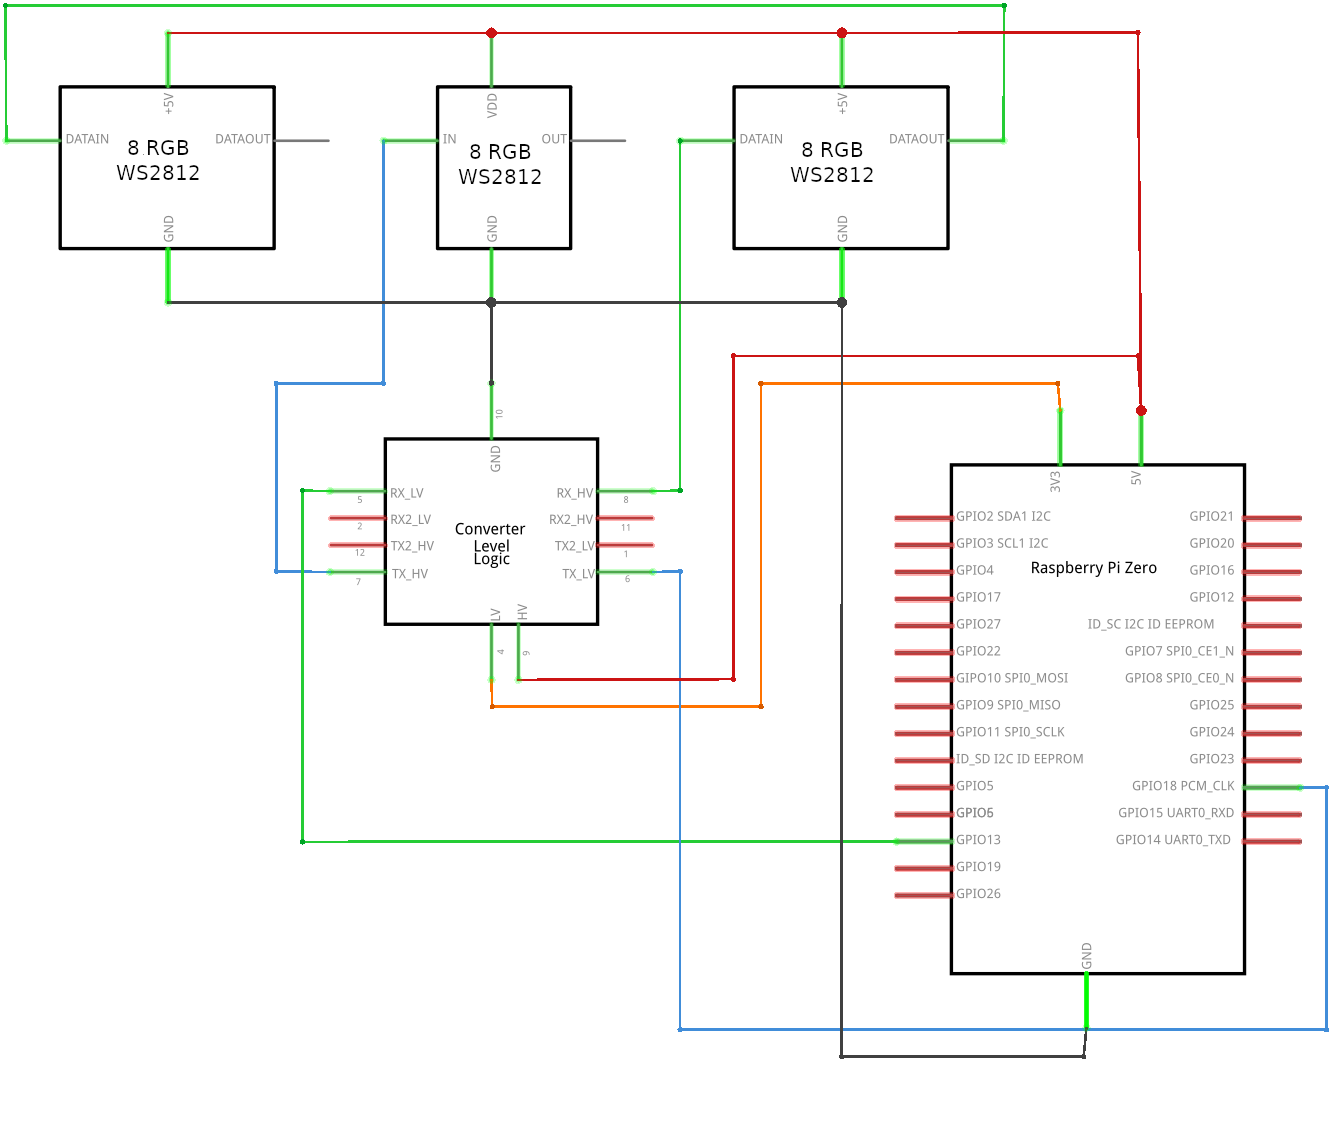
\includegraphics[scale=1]{imaxes/circuito-leds.png}
  \caption{Diagrama de conexión dos LEDs.}
  \label{fig:conexions_leds}
\end{figure}

\section{Cámara}

A cámara a utilizar é a Raspberry Pi Camera, probarase a versión 1 e a versión 2, ambas conectarase a Rasberry Pi Zero co mesmo cable, o conector da placa é delicado polo que deberase conectar con coidado. Para habilitala executarase o comando \emph{raspiconfig} na terminal e no apartado de interfaces activarase a opción cámara.

 Na táboa~\ref{tab:comparativa_camaras} móstrase unha comparativa de ámbalas dúas cámaras e na foto da figura~\ref{fig:camaras} poden verse as tres cámaras a utilizar, a versión 1.3 a versión 2.1 e a 2.1 sen filtro infravermello.
\begin{table}[tbp]
    \label{tab:comparativa_camaras}
    \caption{Táboa comparativa da Raspberry Pi Camera V1 e V2~\cite{mocqRaspberryPiPi2017}}
    \begin{center}
        \begin{tabular}{|l|l||l|}
            \hline
              &  V1 & V2\\ \hline
             Sensor  & 5 Mpíxeles & 5 Mpíxeles \\ \hline
             Resolución foto  & 2592x1944 & 3280x2464 \\ \hline
             Vídeo maxi & 1080p & 1080p \\ \hline
             Tamaño do módulo& 20x25x10 mm & 25x23x9 mm \\ \hline
        \end{tabular}
    \end{center}
\end{table}

\begin{figure}[tbp]
  \centering
  \includegraphics[scale=.06]{imaxes/camaras.jpg}
  \caption{De esquerda a dereita a Raspberry Pi Camera Module V1, V2 sen filtro infravermello e V2 cunha lente de gran angular}
  \label{fig:camaras}
\end{figure}
\subsection{Lentes}
Para poder capturar o completo da estrada a cámara necesitará de algún tipo de lente que permita un maior campo de visión. Existen versións da cámara que xa inclúen unha lente, pero tamén poderemos atopar lentes externas coma es destinadas para os dispositivos móbiles, que contan co tamaño necesario para a cámara da Raspberry. Na figura~\ref{fig:lentes} móstranse as lentes a probar e analizar as tres superiores colocaranse sobre a cámara e as tres inferiores so para a versión da cámara que incorpora lente.
\begin{figure}[tbp]
  \centering
  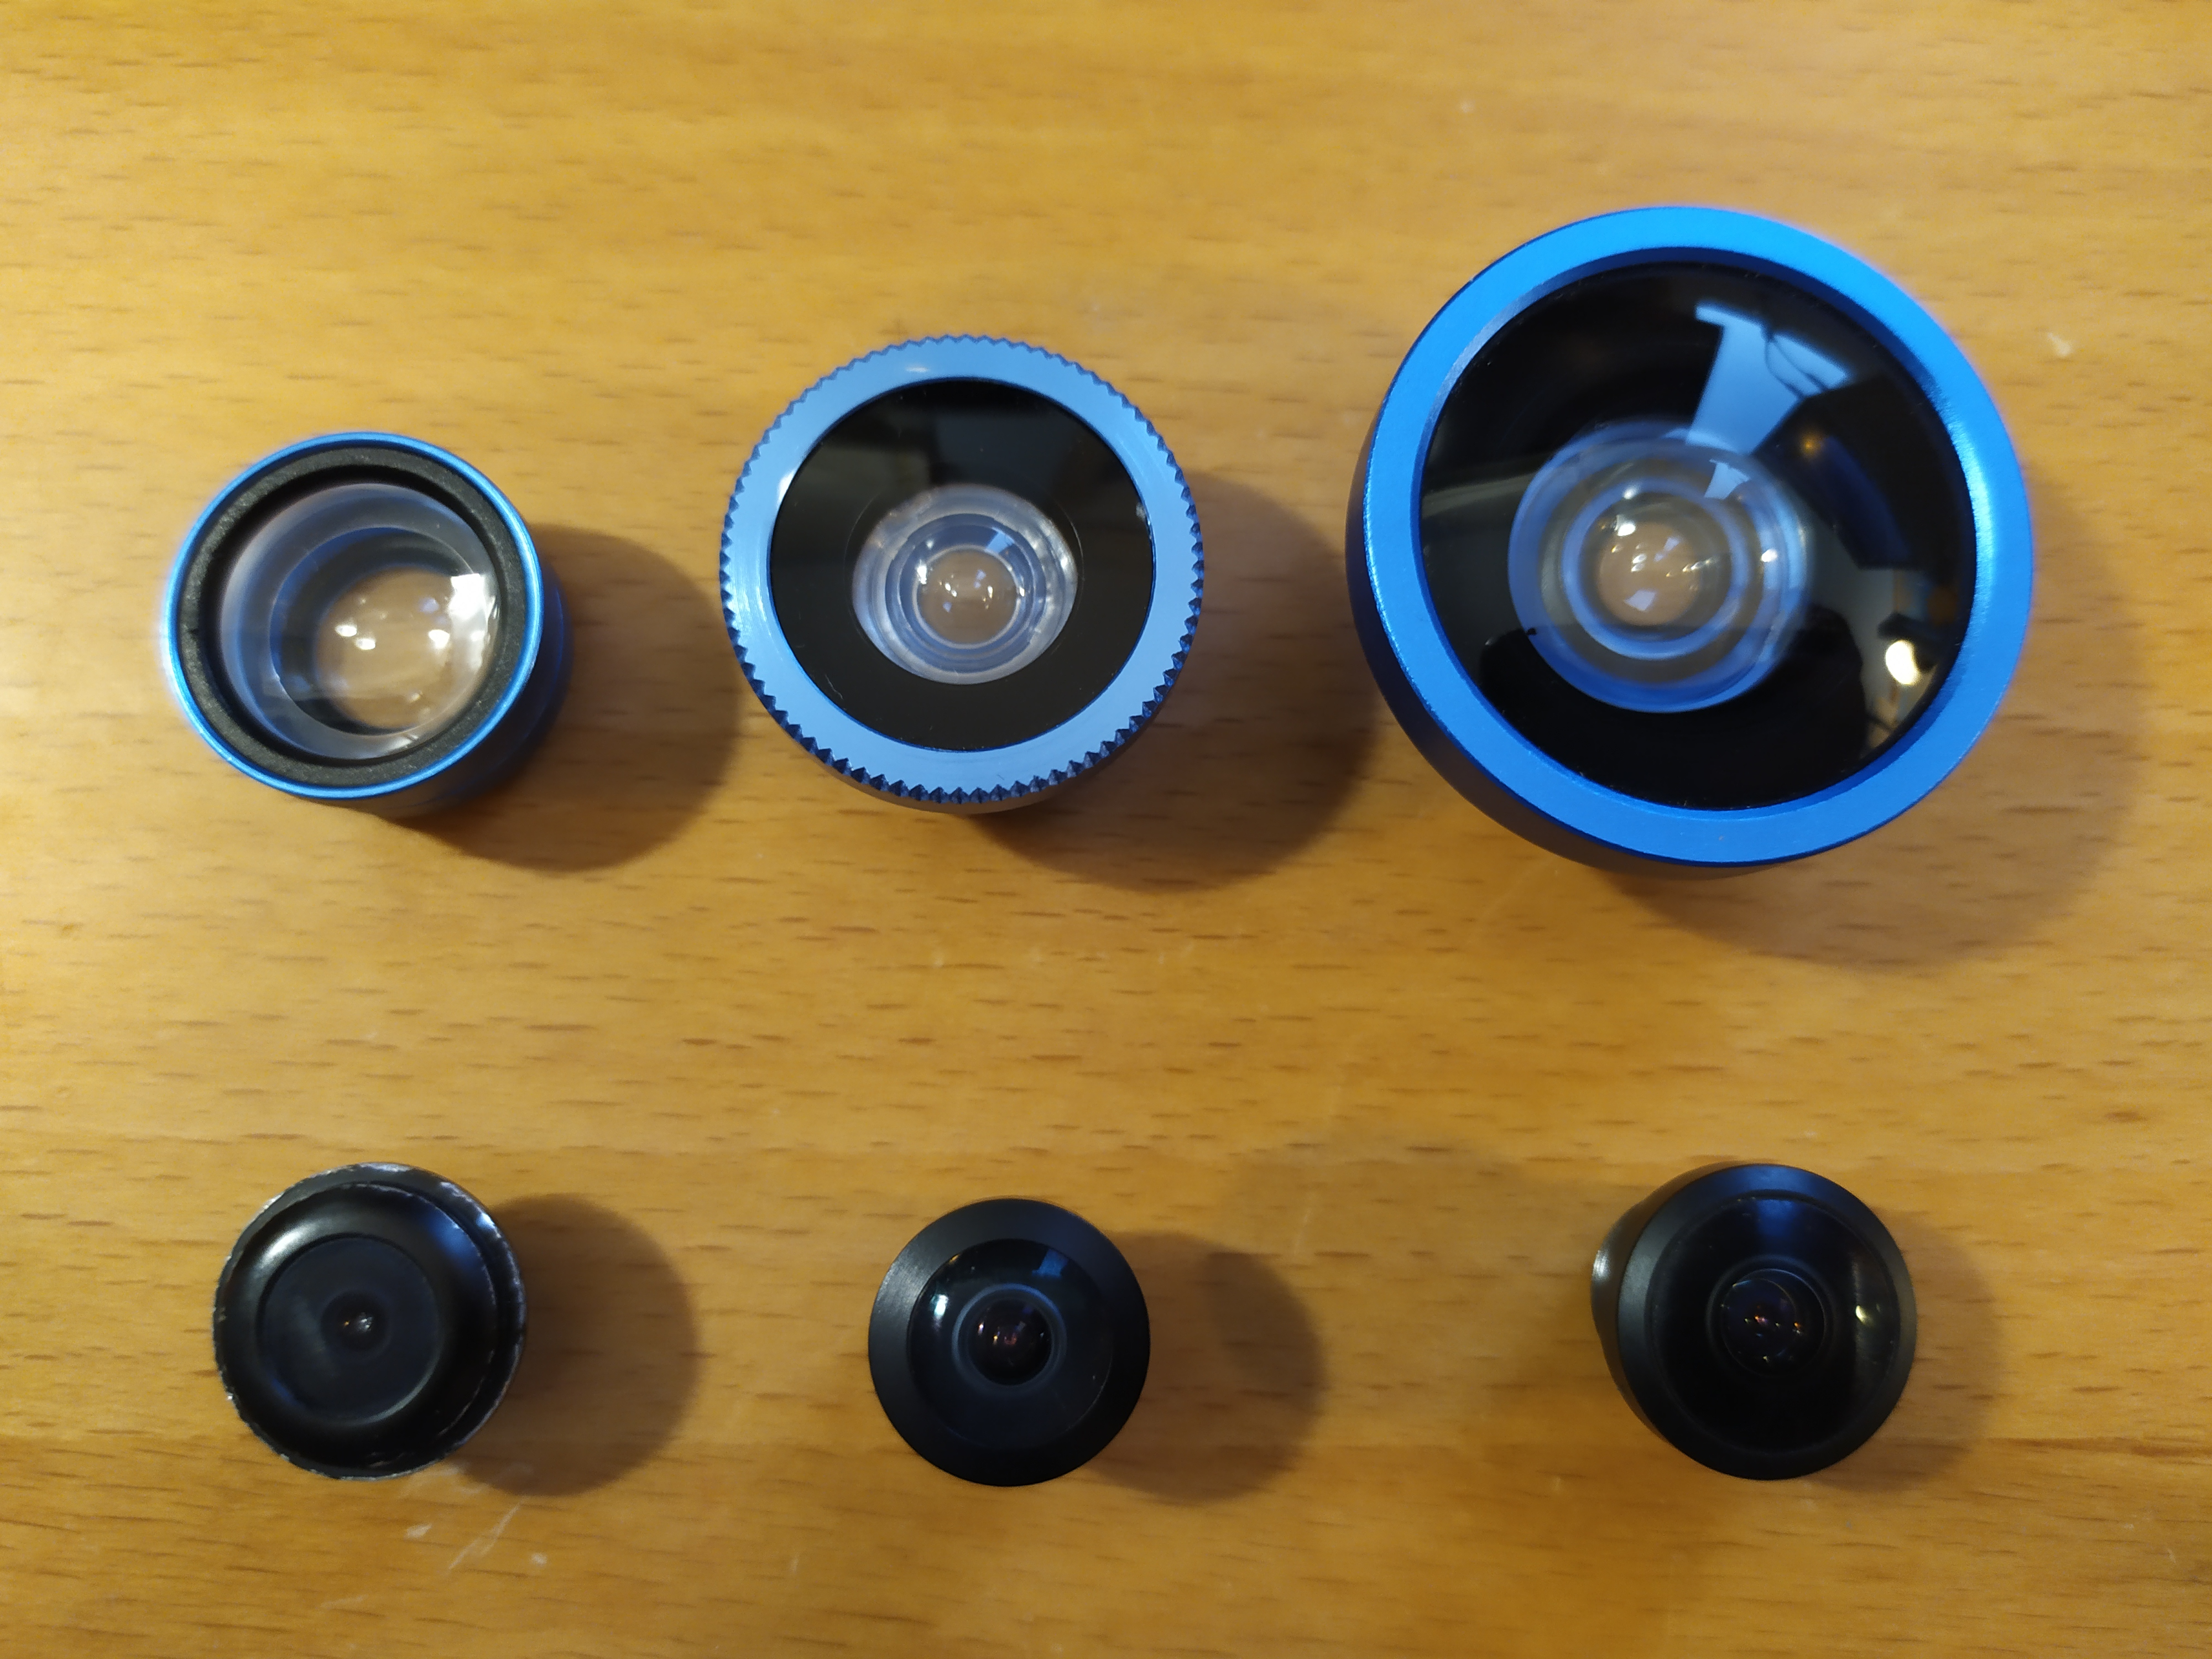
\includegraphics[scale=.06]{imaxes/lentes.jpg}
  \caption{Lentes con diferente ángulo de visión. De esquerda a dereita: fila superior 0.67x, 180º, 0.4x, fila inferior 130º, 160º, 220º }
  \label{fig:lentes}
\end{figure}



\section{Alimentación e enerxía}
O consumo de amperios da Raspberry Pi Zero sen carga de traballo é duns 120 mA, gravando vídeo a 1080p o consumo é de 230mA, gravarase vídeo a 720p polo que o consumo será algo menor pero engadirase o consumo do chip Wi-Fi funcionando. Os LEDs ws2812 teñen un consumo máximo de 60 mA cada un 20 mA como máximo por cada un dos tres LEDs \emph{RGB} a máxima intensidade, o noso máximo consumo realizarse coa luz vermella acesa de forma continua, xa que no resto de modos os padróns de intermitencia reducen o consumo. Contamos con 24 destes LEDs polo que o consumo máximo será de 20mA por 24 LEDs, un total de 480mA que sumados o consumo da Raspberry Pi nos da un consumo máximo teórico de 710mA na versión sen LEDs intermitentes o consumo seria de 160mA máis 230mA, en total 390mA.

\begin{itemize}
    \item Unha primeira versión máis sinxela contará solo cunha batería USB para alimentar a Raspberry. Os requisitos de esta batería serán a amperaxe e a capacidade.

    Partirase do valor do consumo máximo aproximado de 400mA para calcular o tempo de funcionamento. Con esta amperaxe ós 5V que funcionan a Raspberry e os LEDs a potencia utilizada sería de 2W. Neste suposto unha batería de  5000mAh cunha voltaxe nominal de 3.7V pode proporcionar 18.5Wh polo que duraría ata 9 horas e 15 minutos, no caso dunha batería de 1000mAh o tempo mínimo teórico de funcionamento sería de algo menos de dúas horas.
    Comprobaremos se estes supostos se cumpren facendo medicións do tempo de funcionamento.

    \item Realizaremos unha segunda versión máis avanzada que apagará o dispositivo cando a batería baixe de certo limite de voltaxe para evitar que o dispositivo se desconecte e contará tamén cun pulsador para poder acendela e apagala.

    Para isto utilizaremos o chip de carga Adafruit Powerboost 1000 que conta cunhas características moi interesantes a maiores da protección de sobrecarga conta cunha LED e un pin que se activaran cando a voltaxe da batería baixe dos 3.2v, unha voltaxe operacional de 5.2v para evitar perdidas de voltaxe en cables e conectores, un pin habilitador que permite conectar ou desconectar a batería, e proporciona 1 amperio de intensidade sen baixar a voltaxe dos 5v. Non conta con protección de sobrecarga polo que as batería que utilicemos deben incluír un circuíto de protección, este é o caso da maioría de baterías, de utilizar unha sin protección, como unha cela 18650, deberemos engadir o circuíto de protección ou asegurarnos de implementar o apagado por voltaxe baixa correctamente.

    A realización o circuíto basearase no guía \emph{lipopi} de Daniel Bull~\cite{bullGuideSettingLiPo2019} que utiliza o Adafruit Powerboost, nas súas dúas versións a de 500 mA e 1 A, para programar o apagado automático da Rapberry Pi cando a batería baixe de 3.2v e un pulsador para o acendido, tamén conta con dúas versións máis unha que tamén permite o apagado, e outra que monitoriza a voltaxe da batería. Realizarase a versión con pulsador para acendido e apagado.

    O funcionamento é o seguinte, o premer o pulsador conéctase o positivo da batería co pin abilitador, acendendo o adafruit powerboost e por conseguinte acendendo a Raspberry Pi. O acender a Raspberry Pi un pin conectado o pin habilitador acenderase pare seguir mantendo un valor positivo. Para evitar que o voltaxe no pin habilitador caia no tempo entre que pulsamos o pulsador e a Raspberry Pi arranca e encárgase de manter o valor positivo, situaremos un circuíto RC formado por un condensador cunha resistencia en paralelo entre o pulsador e o pin habilitador. O condensador cargarase cando o pulsador cerre o circuíto e descargarase a continuación mantendo a voltaxe o tempo suficiente para que a Raspberry arranque e acenda o pin. Utilizarase un condensador de 100\(\mu\)F xunto cunha resistencia 100k\(\Omega\) que proporcionan un tempo suficiente de 10 segundos. O pin da Raspberry que utilizaremos para este propósito pode ser o 14 correspondente a conexión \emph{uart}, que se acenderá coa Raspberry e se desconectará cando se apague, engadiremos unha resistencia de 10k\(\Omega\) para protexer este pin. Tamén poderíase utilizar calquera outro pin de propósito xeral indicando no arquivo de configuración \emph{config.txt} na partición \emph{boot} da Raspberry, que o pin arranque cun valor positivo e cun valor negativo cando o dispositivo se apague, no caso de utilizar o pin \emph{GPIO} 5 as ordes serían as seguintes: \emph{$gpio=5=op,dh$} para que o pin arranque con valor positivo, \emph{$dtoverlay=gpio-poweroff,gpiopin=5,active_low="y"$} para deixar o pin apagado cando se apaga a Raspberry.

    Para o apagado utilizarase un segundo pin conectado o pulsador, cando este se pulse, estando a Rasberry acesa, se conectará a voltaxe da batería, cando este valor positivo chegue o pin un script Python encargarase de apagar o dispositivo. Engadiranse un divisor de voltaxe para reducir a voltaxe da batería xa que cando está completamente cargada a sua voltaxe de 4.2v e superior o máximo valor lóxico tolerado pola Raspberry Pi de 3.3V. Utilizaremos unha resistencia de 33k\(\Omega\) conectada entre o pin e a batería e unha resistencia de 100k\(\Omega\) entre o pin e terra. Para evitar que o pin de acendido dispare o apagado situarase un díodo entre o pin de acendido e apagado evitando que a voltaxe circule nesa dirección.

    Finalmente conectarase o pin indicador de batería baixa a outro pin de entrada da Raspberry que mediante o script Python apagará o dispositivo. O diagrama de funcionamento mostrase na figura~\ref{fig:circuito_alimentacion}.

    \begin{figure}[tbp]
      \centering
    	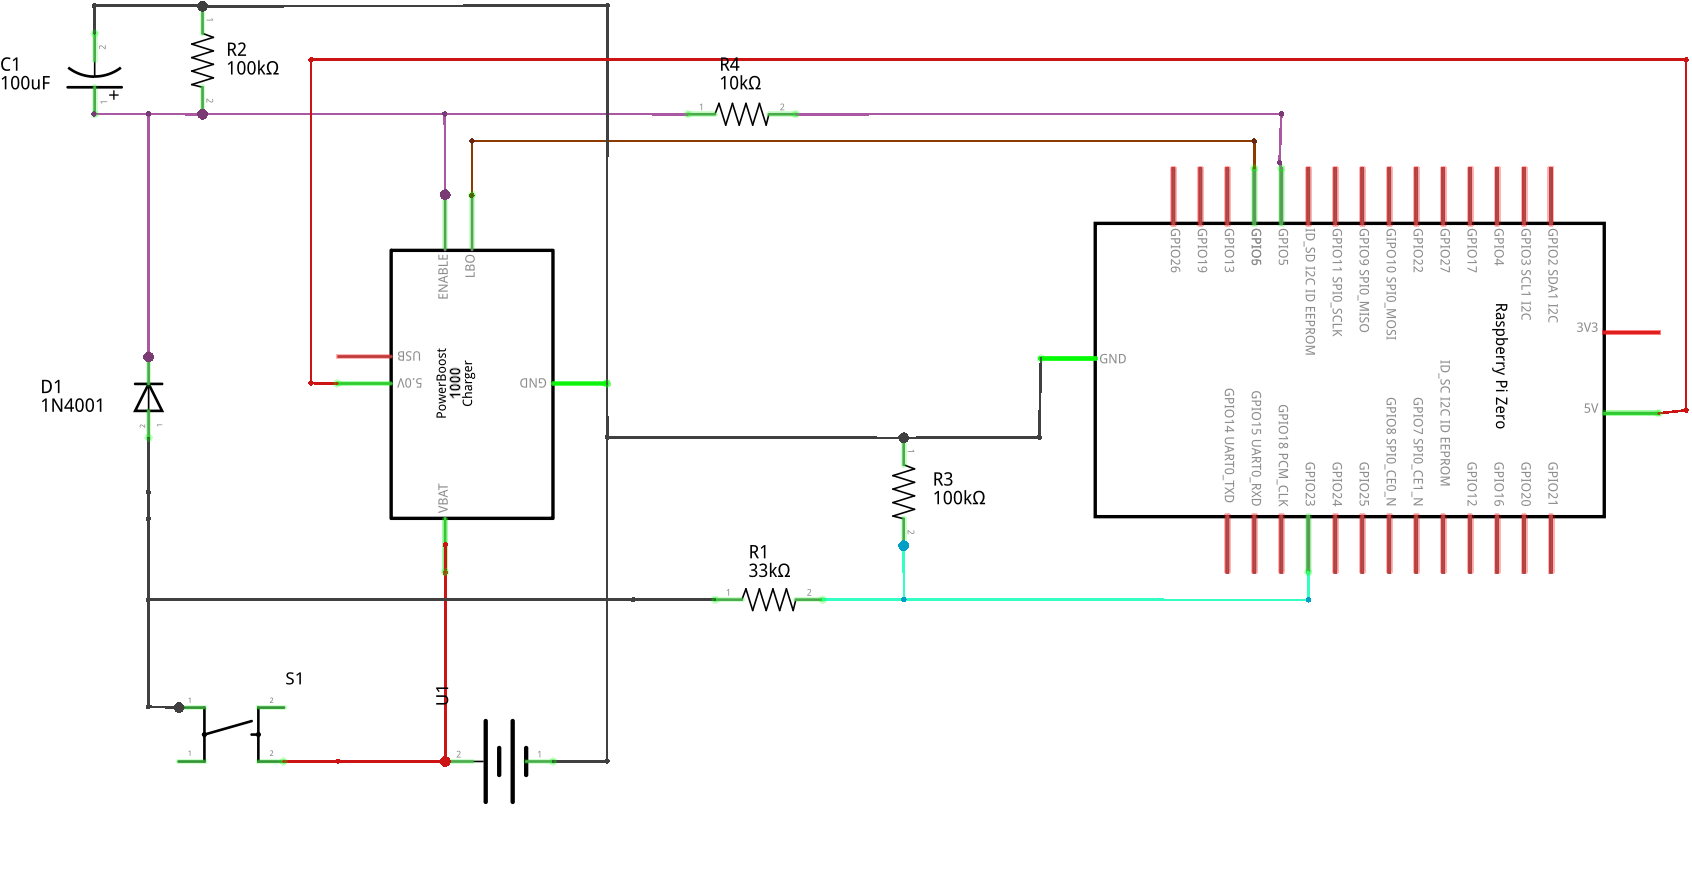
\includegraphics[scale=1]{imaxes/circuito-bateria.png}
    	\caption{Diagrama de funcionamento do circuíto de alimentación.}
    	\label{fig:circuito_alimentacion}
    \end{figure}

    Na figura~\ref{fig:circuito_dispositivo} podemos ver o diagrama final do dispositivo e na figura~\ref{fig:esquema_dispositivo} o esquema completo integrando os LEDs o circuíto de carga e a cámara.

    \begin{figure}[tbp]
      \centering
    	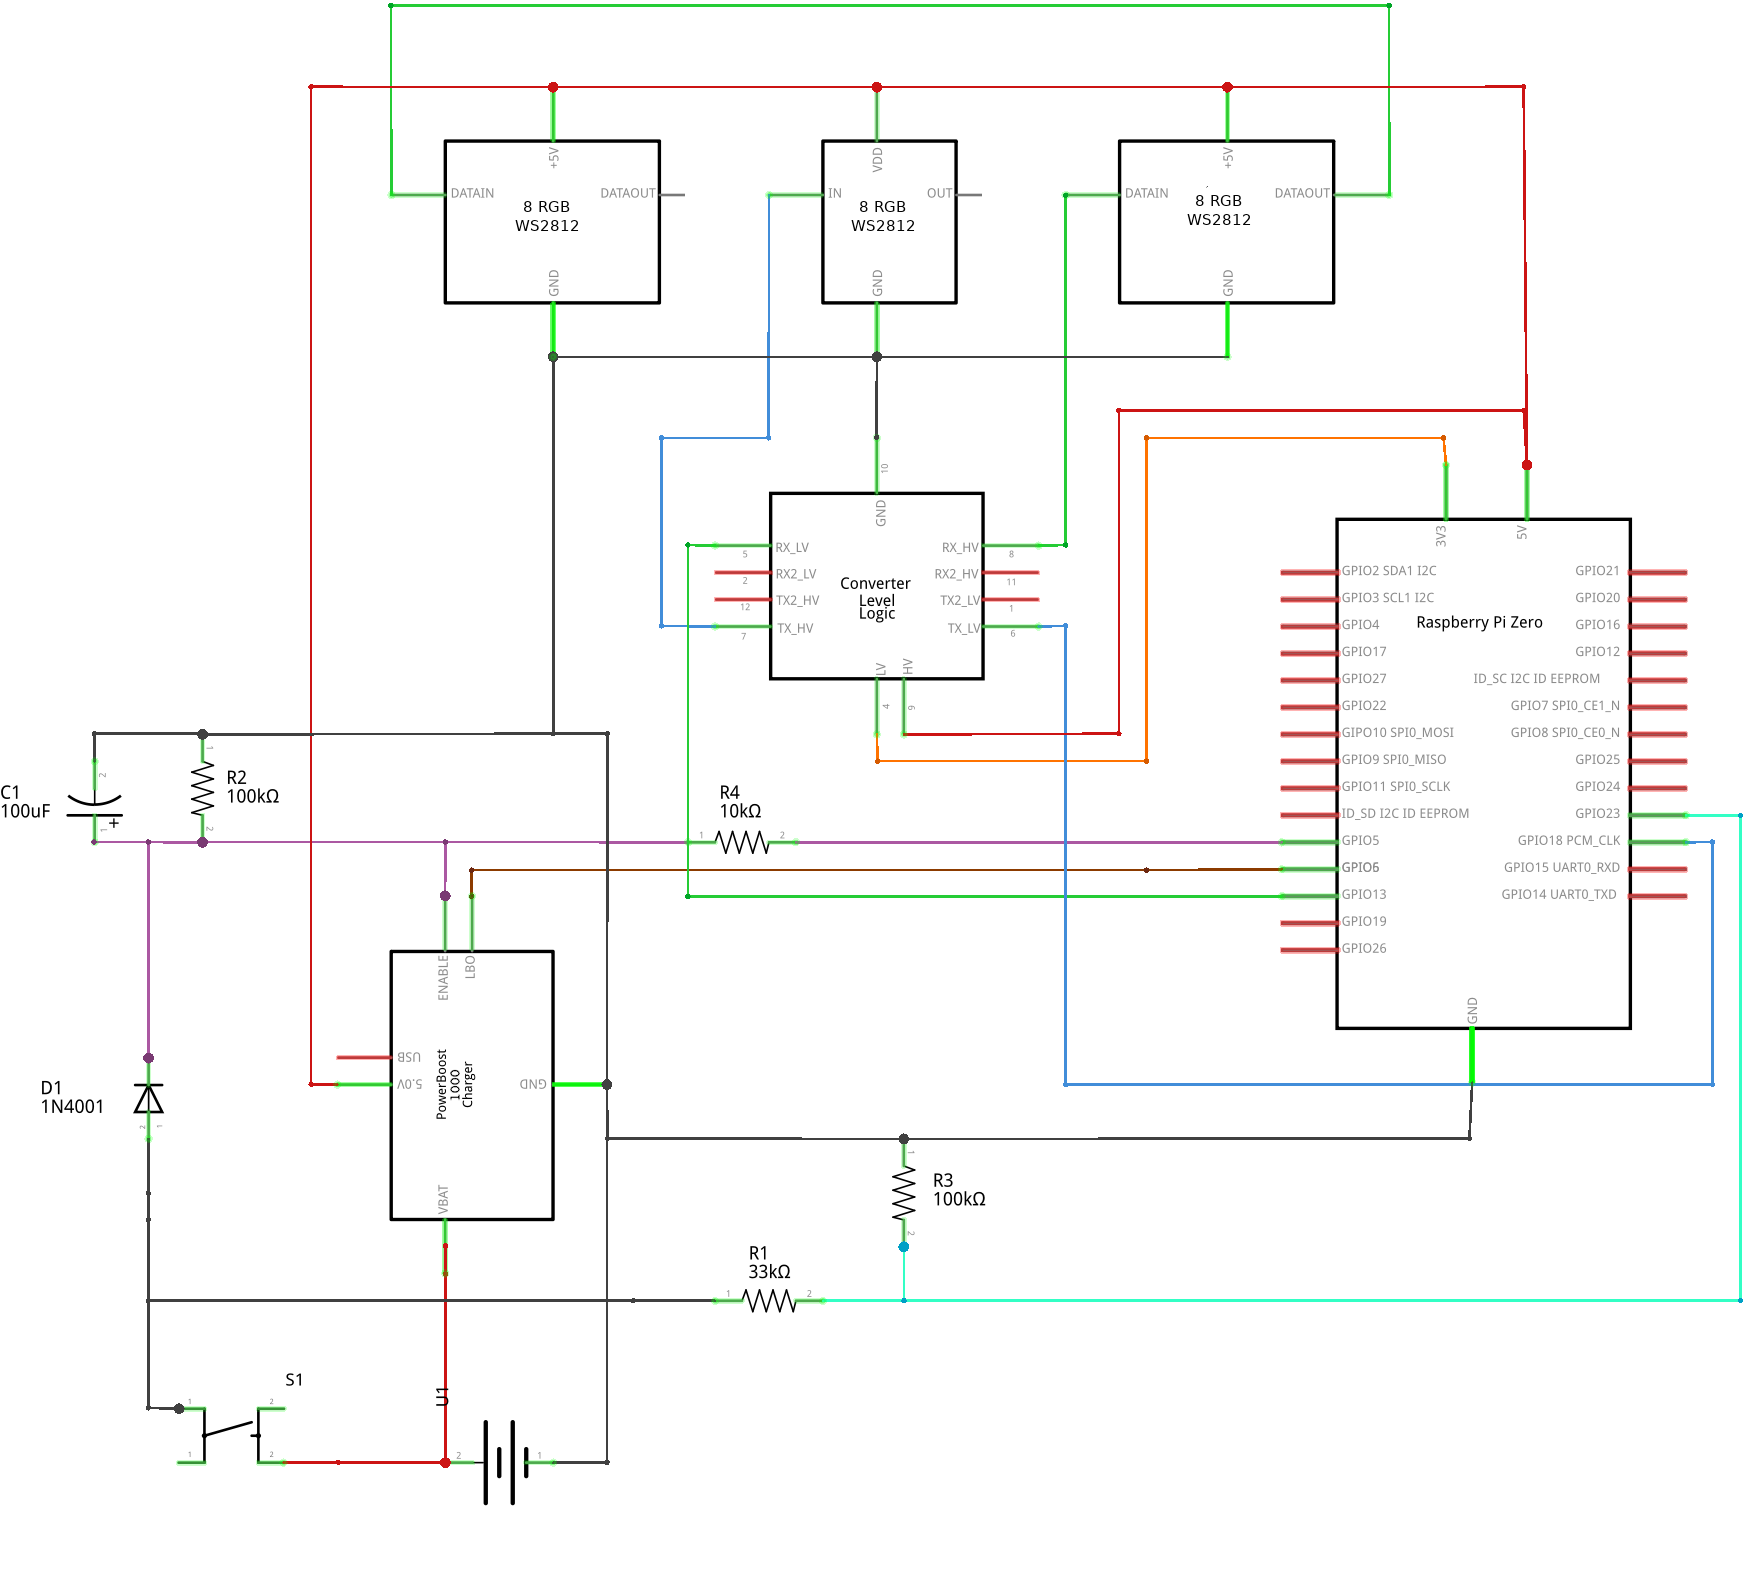
\includegraphics[scale=1]{imaxes/circuito-completo.png}
    	\caption{Diagrama do dispositivo.}
    	\label{fig:circuito_dispositivo}
    \end{figure}

    \begin{figure}[tbp]
      \centering
    	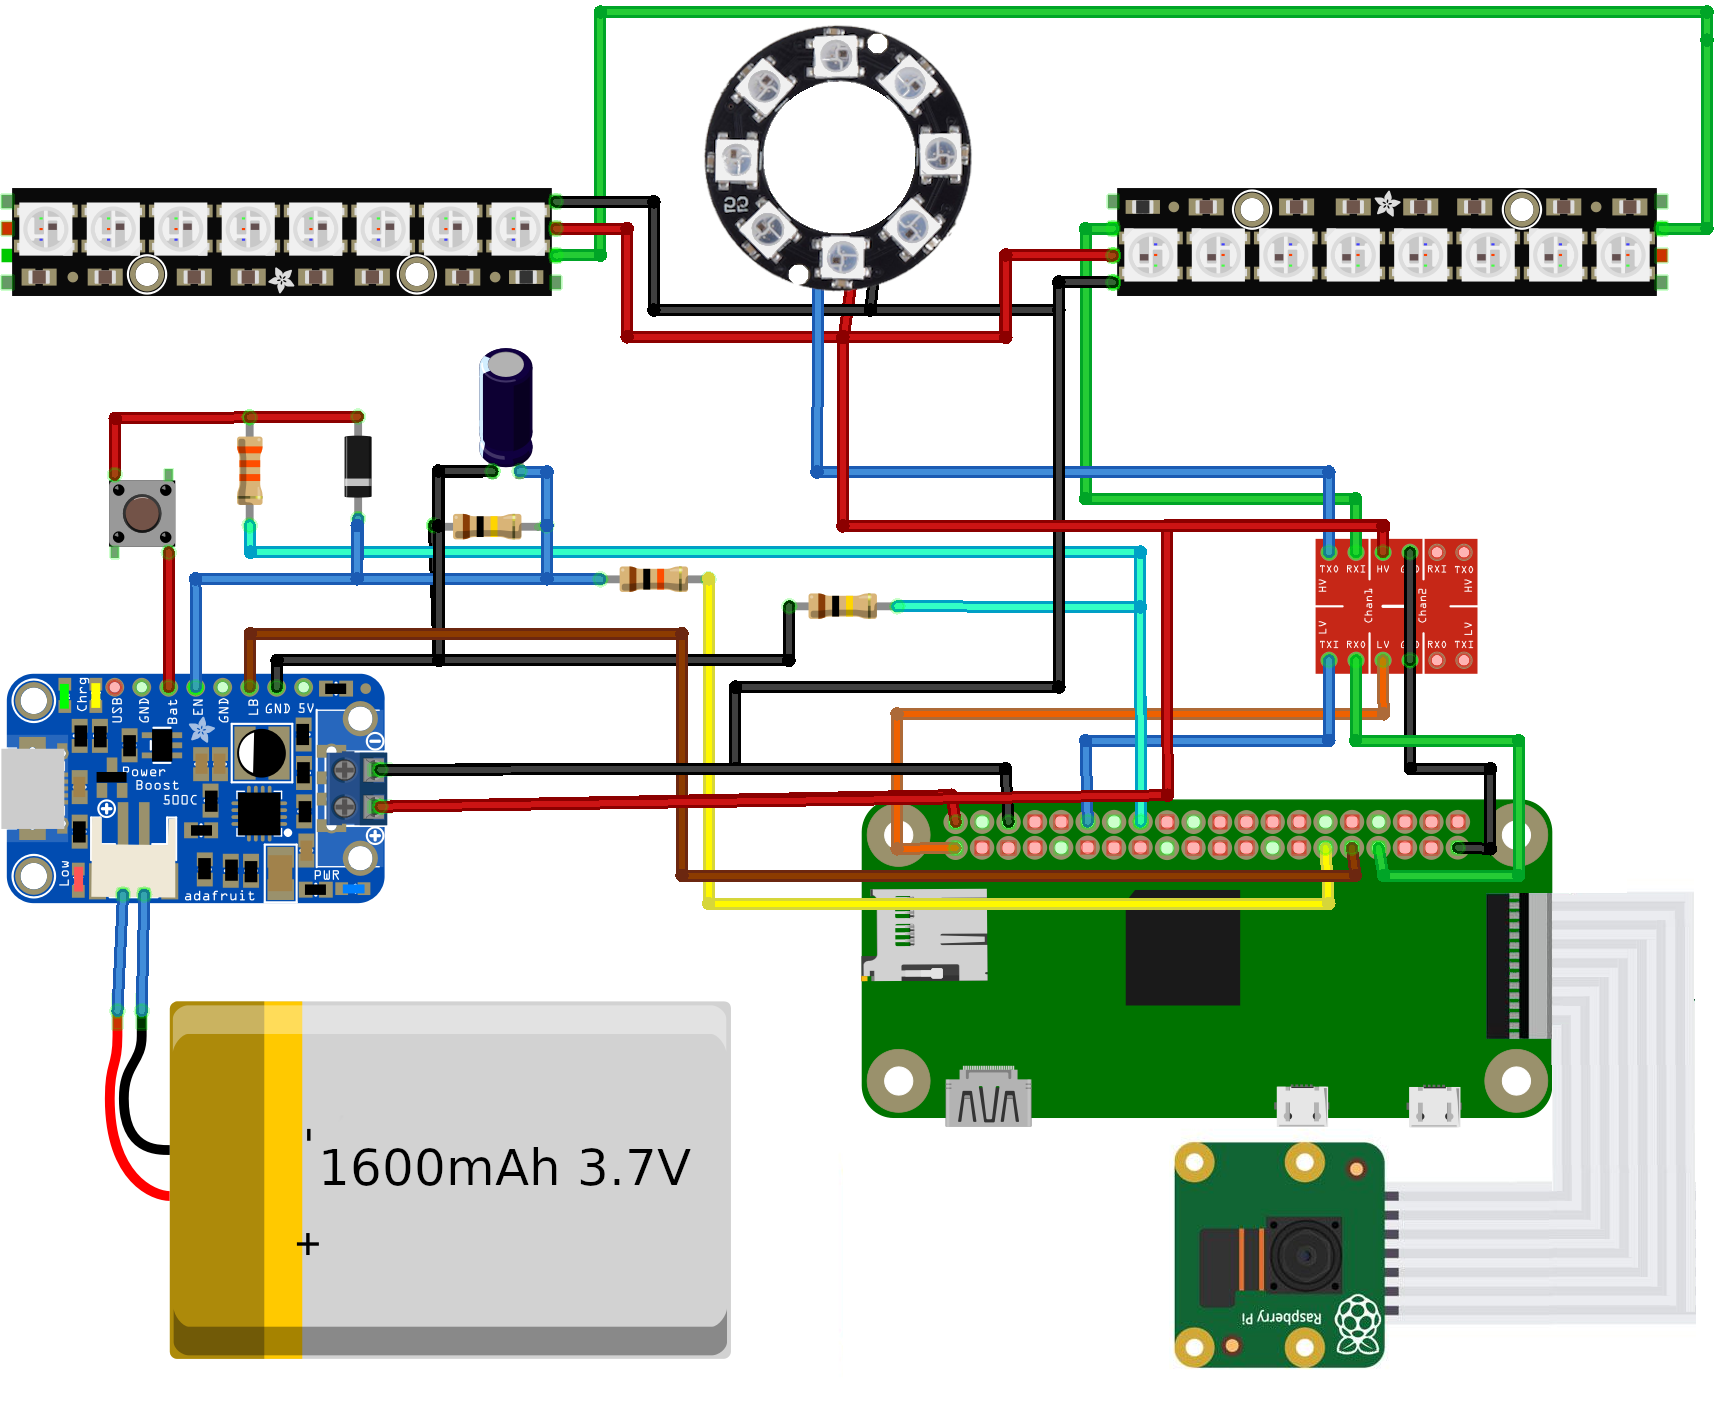
\includegraphics[scale=1]{imaxes/esquema-completo.png}
    	\caption{Esquema completo do dispositivo.}
    	\label{fig:esquema_dispositivo}
    \end{figure}

    Na implementación física colocaremos o chip de carga xunto cos compoñentes electrónicos nunha placa cun conector para poder conectalo directamente os conectores da Raspberry Pi Zero. Tamén colocarase nesta placa o conversor lóxico de nivel como se ve na figura~\ref{fig:fotos_reverso}

    \begin{figure}[tbp]
      \centering
    	\includegraphics[scale=.05]{imaxes/foto-circuito1.jpg}
    	\includegraphics[scale=.05]{imaxes/foto-circuito2.jpg}
    	\caption{Imaxes do circuíto por ambas caras.}
    	\label{fig:fotos_reverso}
    \end{figure}

    Na elección da batería teremos en conta a maiores da sua capacidade o seu tamaño e forma, sendo o ideal que sexa similar o da Raspberry para poder integrala no dispositivo con facilidade. Por eso elixiremos unha batería de 1600mA e 5.92Wh con circuíto de protección e unhas dimensións de 9 x 34 x 50mm que para este suposto, xa que engadindo os LEDs extra calcúlase un consumo máximo de 3.55W, debería proporcionar un tempo mínimo de funcionamento de 2 horas aproximadamente.

\end{itemize}

\section{Software de control de BikeCam}
Nesta sección abordarase todo o software utilizado en BikeCam. Este estruturase en torno o programa Python lightsServer un servidor que se encargará de controlar as luces e executar a orde de transición e parada do video.

No caso de contar cun circuíto de alimentación LipoPi, tamén será necesario ter en funcionamento o script Python LipoPi correspondente.
\subsection{lightsServer}
Este é o servidor principal, as súas funcións son compartir a dirección IP de BikeCam na rede mediante \emph{broadcasting}, inicializar e controlar os LEDs a trabes da libraría rpi\(\_\)ws281x, aceptar conexións de BikeView e recibir, executar e confirmar as súas oredes.
\subsubsection{Broadcasting da dirección IP}
Os dispositivos conectaranse mediante unha rede local, xa sexa a través dun cable USB ou dunha rede Wi-Fi, en ámbolos dous casos o dispositivo Android será o encargado de aloxar a rede xa sexa compartindo por USB ou creando un punto de aceso Wi-Fi.

En canto arranque o servidor execútase a función encargada de \emph{broadcastear} cada 3 segundos unha mensaxe co texto "BikeView" a dirección de \emph{broadcast} mediante un \emph{datagram socket}. Esta función deterase se o servidor acepta unha conexón entrante. No momento que se peche a conexión, chamarase a función de novo e seguirase \emph{broadcasteando} a espera dunha nova conexión.

\section{Recepción de ordes}
 Para recibir os comandos enviados dende o dispositivo móbil e executalos mediante Python implementaremos un servidor tamén Python para poder integrar a recepción e a execución de ordes no mesmo programa.

 A primeira opción será utilizar peticións \emph{http} e manexalas mediante a clase de Python \emph{BaseHTTPRequestHandler}, o problema é que esta clase bloquea o programa mentres se executan as ordes correspondentes a petición recibida. Para solucionar este problema poderiáse implementar un servidor \emph{multithread} ou utilizar unha libraría para Python que implemente o servidor \emph{multithread} de forma transparente. Plantexase utilizar as librarias \emph{multithread} \emph{Tornado}, \emph{Twisted} ou \emph{lighttpd} pero debido os recursos limitados da Rasberry Pi Zero o uso dunha destas librarías podería implicar maiores latencias e consumo enerxético.

 Finalmente optase por manexar a conexión directamente mediante \emph{sockets} non bloqueastes é así poder utilizar un solo \emph{thread}. Para elo introduciremos as peticións de conexión nunha lista, unha vez aceptada introducirase nunha segunda lista as mensaxes recibidas e se executara a orde correspondente para cada mensaxe.

\subsubsection{Xestión dos LEDs}
Para manexar os LEDs utilizaremos a libraría rpi\(\_\)ws281x de Jeremy Garff~\cite{garffUserspaceRaspberryPi2019} na sua versión para Python. O seu funcionamento é moi simple, primeiro teremos que configurar os parámetros da tira LED, coma o numero de LEDs, o pin a que esta conectado, o tipo de tira  ou a canle \emph{PWM} entre outros. No programa principal deberemos inicializar os LEDs con estes parámetros e executala coa función \emph{begin}. Cada vez que queiramos que os les cambien os seu estado chamaremos a función \emph{show}.

Escribiranse funcións encargadas dos padróns de iluminación. Estes padróns serán os seguintes:
\begin{itemize}
    \item \textbf{Luz vermella fixa},
    É a encargada de indicar a posición da bicicleta.
    \item \textbf{Luz vermella intermitente},
    A sua función é a mima que a anterior, pero o padrón de intermitencia aumentara a visibilidade. Crearanse distintos padróns combinando distintas frecuencias en intensidades lumínicas.
    \item \textbf{Luz vermella incremental},
    É a encargada de indicar a freada, a sua intensidade aumentará ata o valor máximo para emular as luces de freada dos coches.
    \item \textbf{Luz amarela de xiro a esquerda ou dereita},
    Indica o xiro iluminando progresivamente os LEDs do anel dende os situados no centro ata os do estremo esquerdo ou dereito, de dispoñer das tiras extra de LEDs de xiro estas iluminaranse a continuación. Unha vez iluminados tódolos LEDs estes se apagarán e o padrón repetirase de novo.
\end{itemize}

Tamén se escribirá unha función para controlar a intensidade dos LEDs en función dun valor numérico recibido, 0 será mínimo e 9 a máxima intensidade.


\subsection{Captura de vídeo}
\emph{Raspivideo} é o software que utilizaremos para capturar as imaxes, o programa executase dende terminal proporcionándolle diferentes parámetros. No noso caso os parámetros a utilizar serán:
\begin{itemize}
    \item -t Tempo de captura de vídeo, no noso caso será 0 indicando que a captura será continua.
    \item -w e -h Son os parámetros de anchura e altura de píxeles, probaremos diferentes resolucións para conseguir a máxima calidade posible sempre que o tamaño da imaxe non repercuta na latencia de transmisión.
    \item -fps \emph{Frames per second}, é o numero de imaxes a capturar cada segundo, variaremos con este valor para minimizar a latencia.
    \item -b \emph{Bitrate}, o numero de bits por segundo, buscaremos o valor máis alto posible sen que produza retardos na transmisión.
    \item -n Con este parámetro deshabilitaremos a previsualización do vídeo.
    \item -pf Parámetro para elixir o perfil do codificador de vídeo H264, as opcións dispoñibles son, \emph{baseline}, \emph{main} and \emph{high}. Utilizaremos a opción \emph{baseline} xa que é a que menor custo computacional ten.
    \item -o Con este parámetro indicamos a saída de vídeo, como por exemplo a un arquivo, no noso caso utilizaremos a saída estándar que indicaremos con "-" , e que redirecionaremos máis tarde.
\end{itemize}
\subsection{Transmisión de vídeo}
Para transmitir o vídeo ao dispositivo móbil a través da rede preséntanse varias posibilidades. Para comparalas transmitiremos vídeo dende a Raspberry Pi cunha mesma resolución, 720p, e o recibiremos e o reproduciremos nun pc mediante \emph{vlc}.

\begin{itemize}
    \item A primeira opción a analizar é o software de vídeo \emph{vlc}, unha completa ferramenta de reprodución que tamén permite a transmisión e a recepción de vídeo na rede mediante diferentes protocolos. Faremos unha proba utilizando o \emph{vlc} na Raspberry Pi para transmitir o vídeo da cámara e recibilo nun pc con \emph{vlc}. Como resultado obtemos unha transmisión cunha latencia superior a un segundo, que imposibilita o seu uso para controlar o trafico en tempo real.

    \item A segunda opción que probaremos consistirá en capturar o vídeo coa ferramenta de captura de vídeo da Raspberry Pi, \emph{raspivid}, e redirecionar a sua saída a rede utilizando \emph{netcat} unha utilidade para transmitir e recibir na rede mediante \emph{tcp} ou \emph{udp}. Transmitiremos mediante \emph{udp} para conseguir unha menor latencia a custo de perder algún fotograma. A recepción de vídeo a realizaremos nun pc mediante \emph{vlc} coma no caso anterior. A latencia obtida neste caso e mellor que no anterior.

    \item Buscando reducir aínda máis a latencia probaremos a utilizar o software \emph{socat}, que funciona de forma similar a \emph{netcat} e conta tamén con moitas opcións de configuración. O procedemento será igual que no caso anterior, faremos a captura con \emph{raspivid} e redirecionaremos o vídeo a un porto nunha dirección \emph{ip} mediante \emph{udp} neste caso utilizando \emph{socat}. Como resultado obtemos unha latencia aínda menor que con \emph{netcat} polo que utilizaremos este software para a transmisión de vídeo.
\end{itemize}
\subsection{LipoPi}
Este é un script Python encargado de comunicar a Raspberry Pi co circuíto de carga. As súa función é enviar unha orde de apagado o sistema que cerrará tódolos programas, incluíndo LightsServer e apagará o sistema. Para isto rexistra unha función de \emph{callback} que se executará cando se produce un cambio nun dos seguintes pins.
\begin{itemize}
  \item  O pin conectado a liña de baixo voltaxe do Adafruit Powerboost, que poñerase a 0 cando batería estea baixa.
  \item  O pin conectado o pulsador, que tomara un valor positivo cando se prema e cerre o circuíto.
\end{itemize}
Tamén xenera un arquivo de logs no que informará do motivo e o momento de cada apagado.
\subsection{Servizos en \emph{sytemd}}
    Estes servizos executan unha programa cando arranca o sistema e o reinicia cada vez que se pechen se así o indicamos. A súa estrutura e sinxela nela se indica a orde de execución a iniciar, e a ubicación do arquivo, tamén se lle poden indicar outros parámetros como se se quere que se reinicie sempre se se pecha, o tempo de espera en caso de reinicio do programa ou o momento de execución cando o sistema arranca.
    Para instalar un novos servizo se copiaría o arquivo \emph{.service} a ubicación \emph{/etc/systemd/system/} despois se abilitaría coa orde \emph{systemctl enable nomeDoServizo} e se iniciaría coa orde  \emph{systemctl enable nomeDoServizo}
    \subsubsection{bikecam service}
    Este servizo executase co arranque do sistema e arranca ao servidor LightsServer despois de que se cargue as interfaces de rede.
    \subsubsection{lipopi service}
    Para arrancar automaticamente o script Python instalarase un novo servizo en \emph{sytemd} e de igual maneira que co servidor executarase no arranque e cada vez que se pare.

\section{Carcasa e ancoraxe}

Para protexer o dispositivo e suxeitalo baixo a sela da bicicleta plantexaranse dúas opcións.

    \subsection{Versión con batería externa}

    A primeira realizarase para a versión do proxecto alimentada cunha batería USB. Consistirá en utilizar a carcasa oficial da Raspberry Pi Zero que inclúe un oco para a cámara e espazo para as conexión na parte de atrás, a carcasa so permite a uso de cámaras sen lentes polo que incorporarase unha lente externa.

    Para suxeitar a carcasa á bicicleta deseñaremos un soporte en 3d co software Blender. Partiremos das medición da carcasa e deseñarase un soporte que suxeite a carcasa firmemente e permita atala a barra da sela mediante unha correa.

    Unha vez deseñado e tras comprobar que o deseño e imprimible exportarase no formato \emph{STL} que abrirase cun software encargado de dividir o deseño en capas e traducilo a ordes de desprazamento interpretables pola impresora, aquí configuraranse diferentes parámetros como a altura de capa, que é a resolución de impresión, as velocidades, a cantidade e tipo de recheo da peza ou o uso de soportes para facilitar a impresión. Neste caso utilizaras o software libre Slic3r no que configurarase a peza a imprimir cun 100\(\%\) de recheo para que sexa máis sólida cunha altura de capa de 0.2mm e sen uso de soportes, como resultado obterase un arquivo \emph{GCODE}  que pasaremos a impresora. O prototipo imprimirase o prototipo en 3d probarase e aplicaranse correccións no modelo. Para este deseño realizáronse dúas iteracións móstranse na figura~\ref{fig:soporte_caixa}.

    \begin{figure}[tbp]
      \centering
      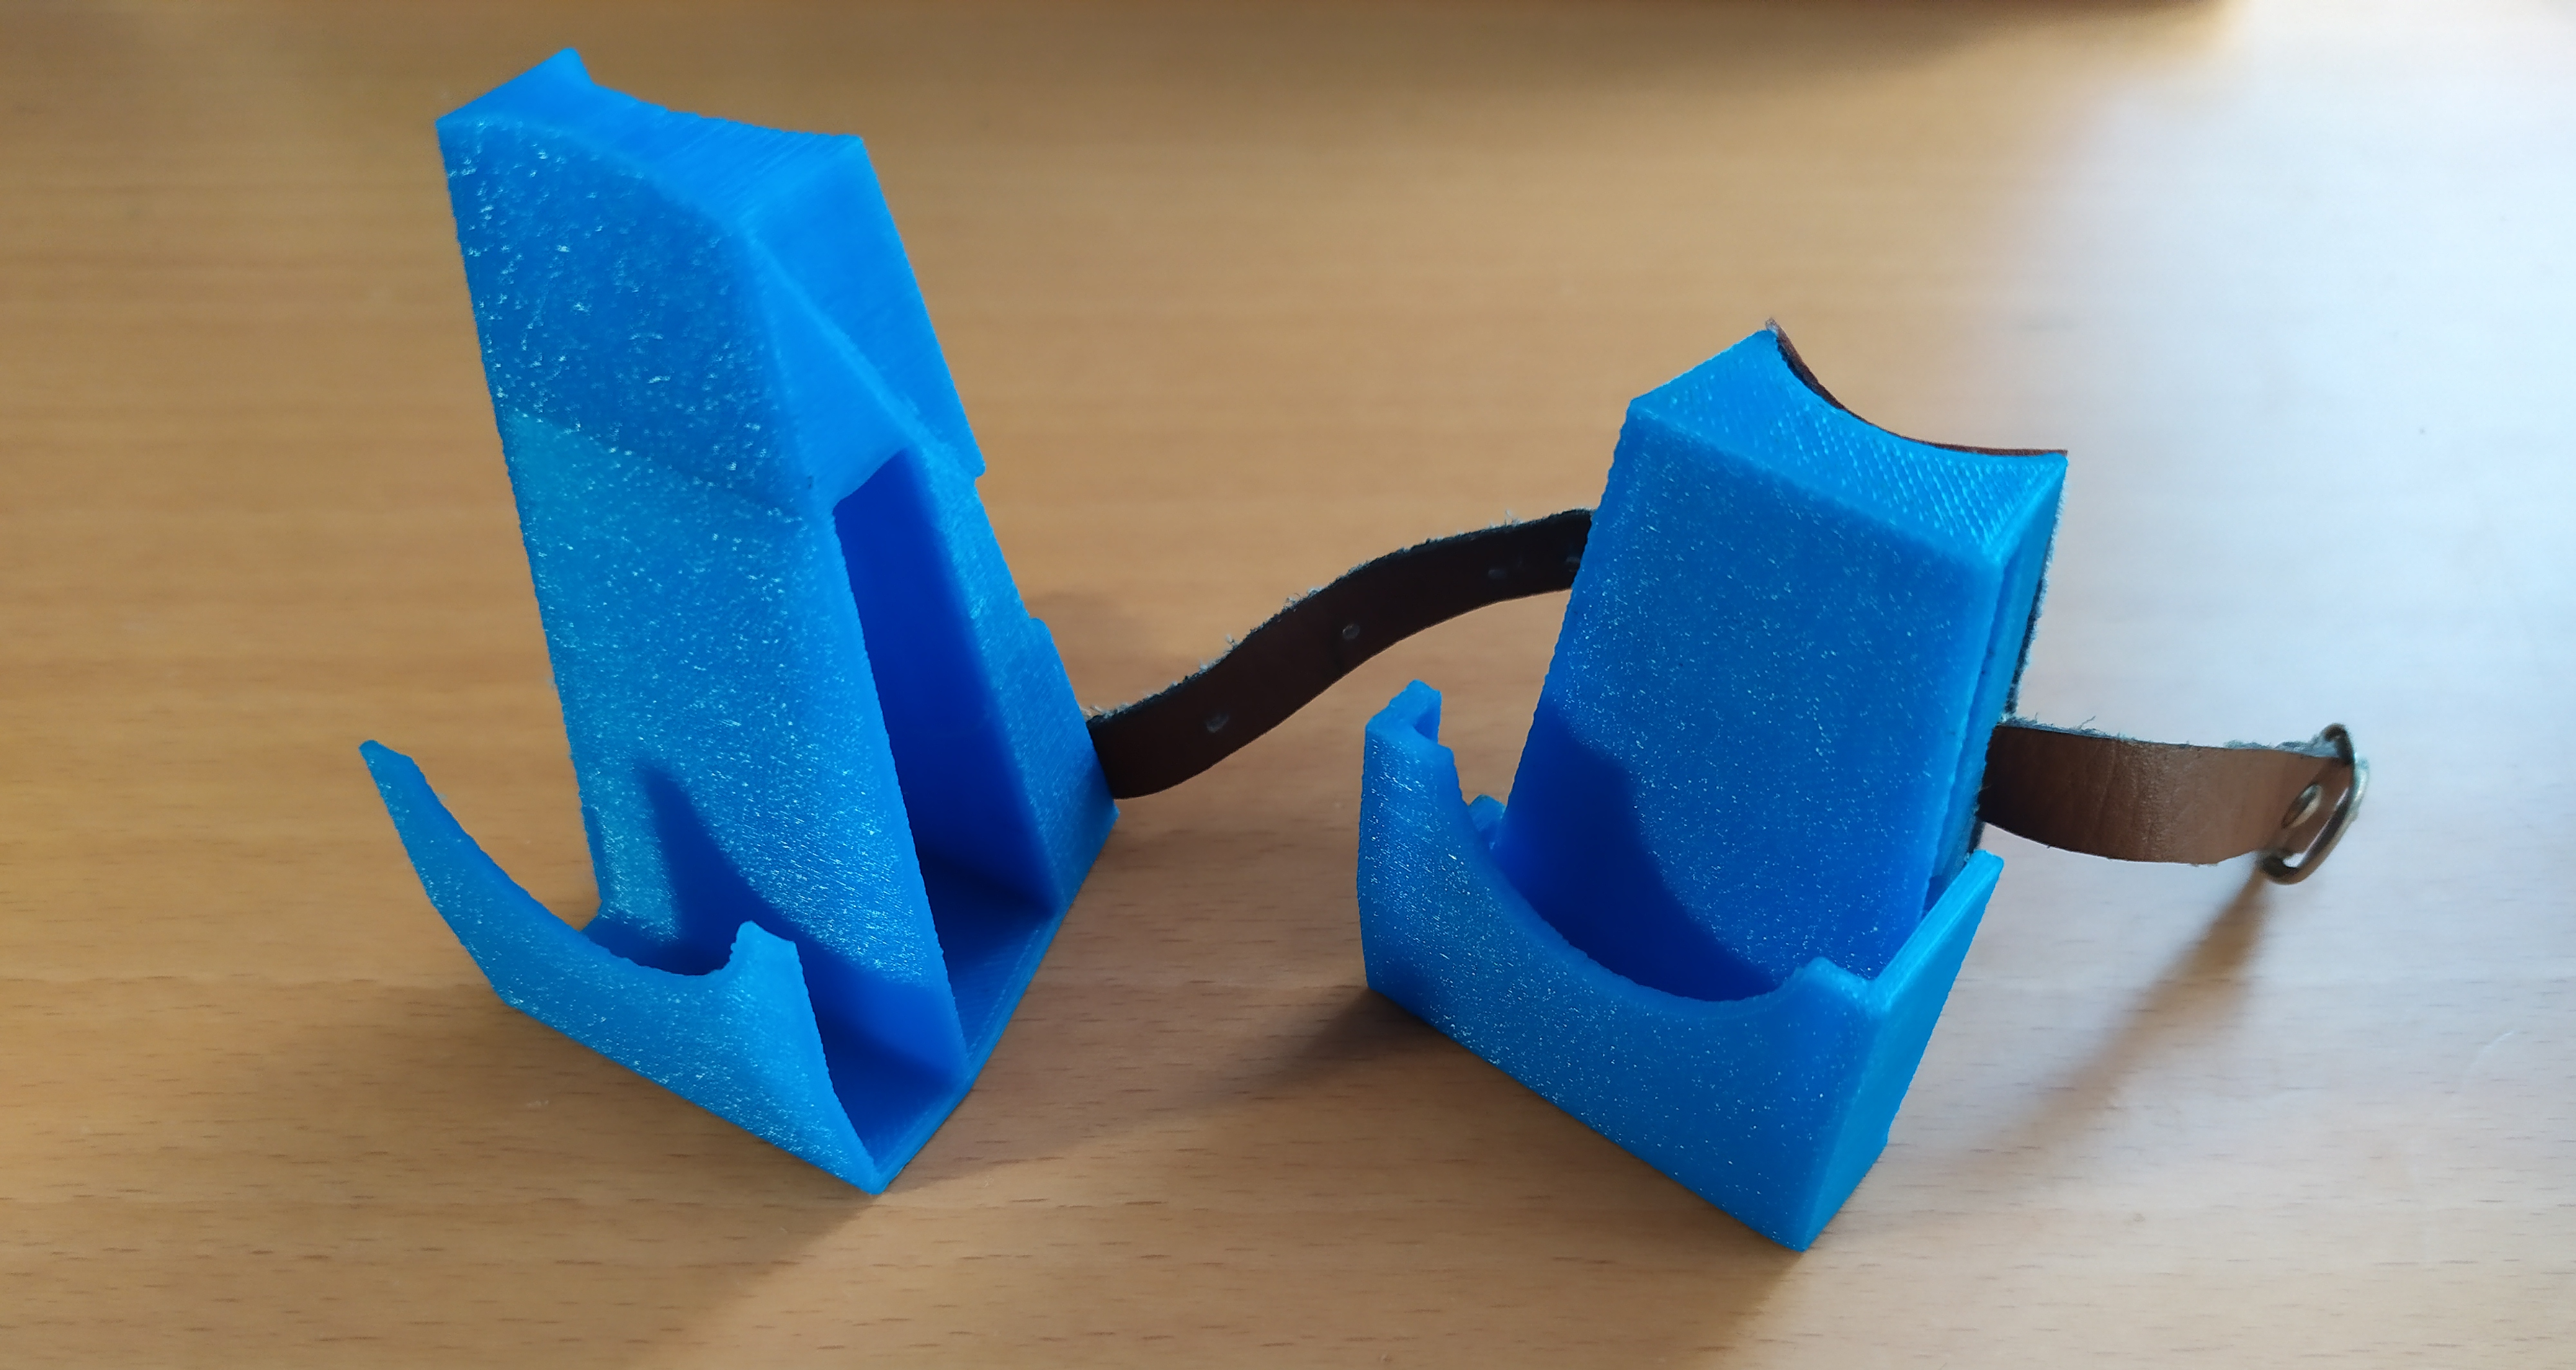
\includegraphics[scale=.1]{imaxes/soporte-caixa.jpg}
      \caption{Deseños do soporte na bicicleta para a caixa oficia da Rasberry Pi.}
      \label{fig:soporte_caixa}
    \end{figure}


    \subsection{Versión con batería interna}
    A segunda versión terá que albergar a Raspberry Pi Zero xunto coa cámara, o chip de carga e alimentación, o conversor lóxico de voltaxe e a batería. Utilizaremos tamén neste caso o software de edición 3d Blender para deseñar os prototipos.

    O deseño contara co anel LED situado no exterior o redor da lente da cámara, no interior colocaranse tódolos compoñentes electrónicas e a batería. Na parte superior contará cun oco para o conector micro USB de carga e aceso a tarxeta micro sd da Raspberry Pi. No exterior contará tamén con dous brazos articulados nos que situaremos as dúas tiras LEDs para indicar o xiro.

    Da mesma forma que no caso anterior o deseño imprimirase modificarase e volverase a imprimir ata que se obteña un resultado aceptable. Na figura~\ref{fig:evolucion_carcasa} pódese observar a evolución dos diferentes deseños e na figura~\ref{fig:carcasa} unha imaxe renderizada do deseño final.


    \begin{figure}[tbp]
      \centering
      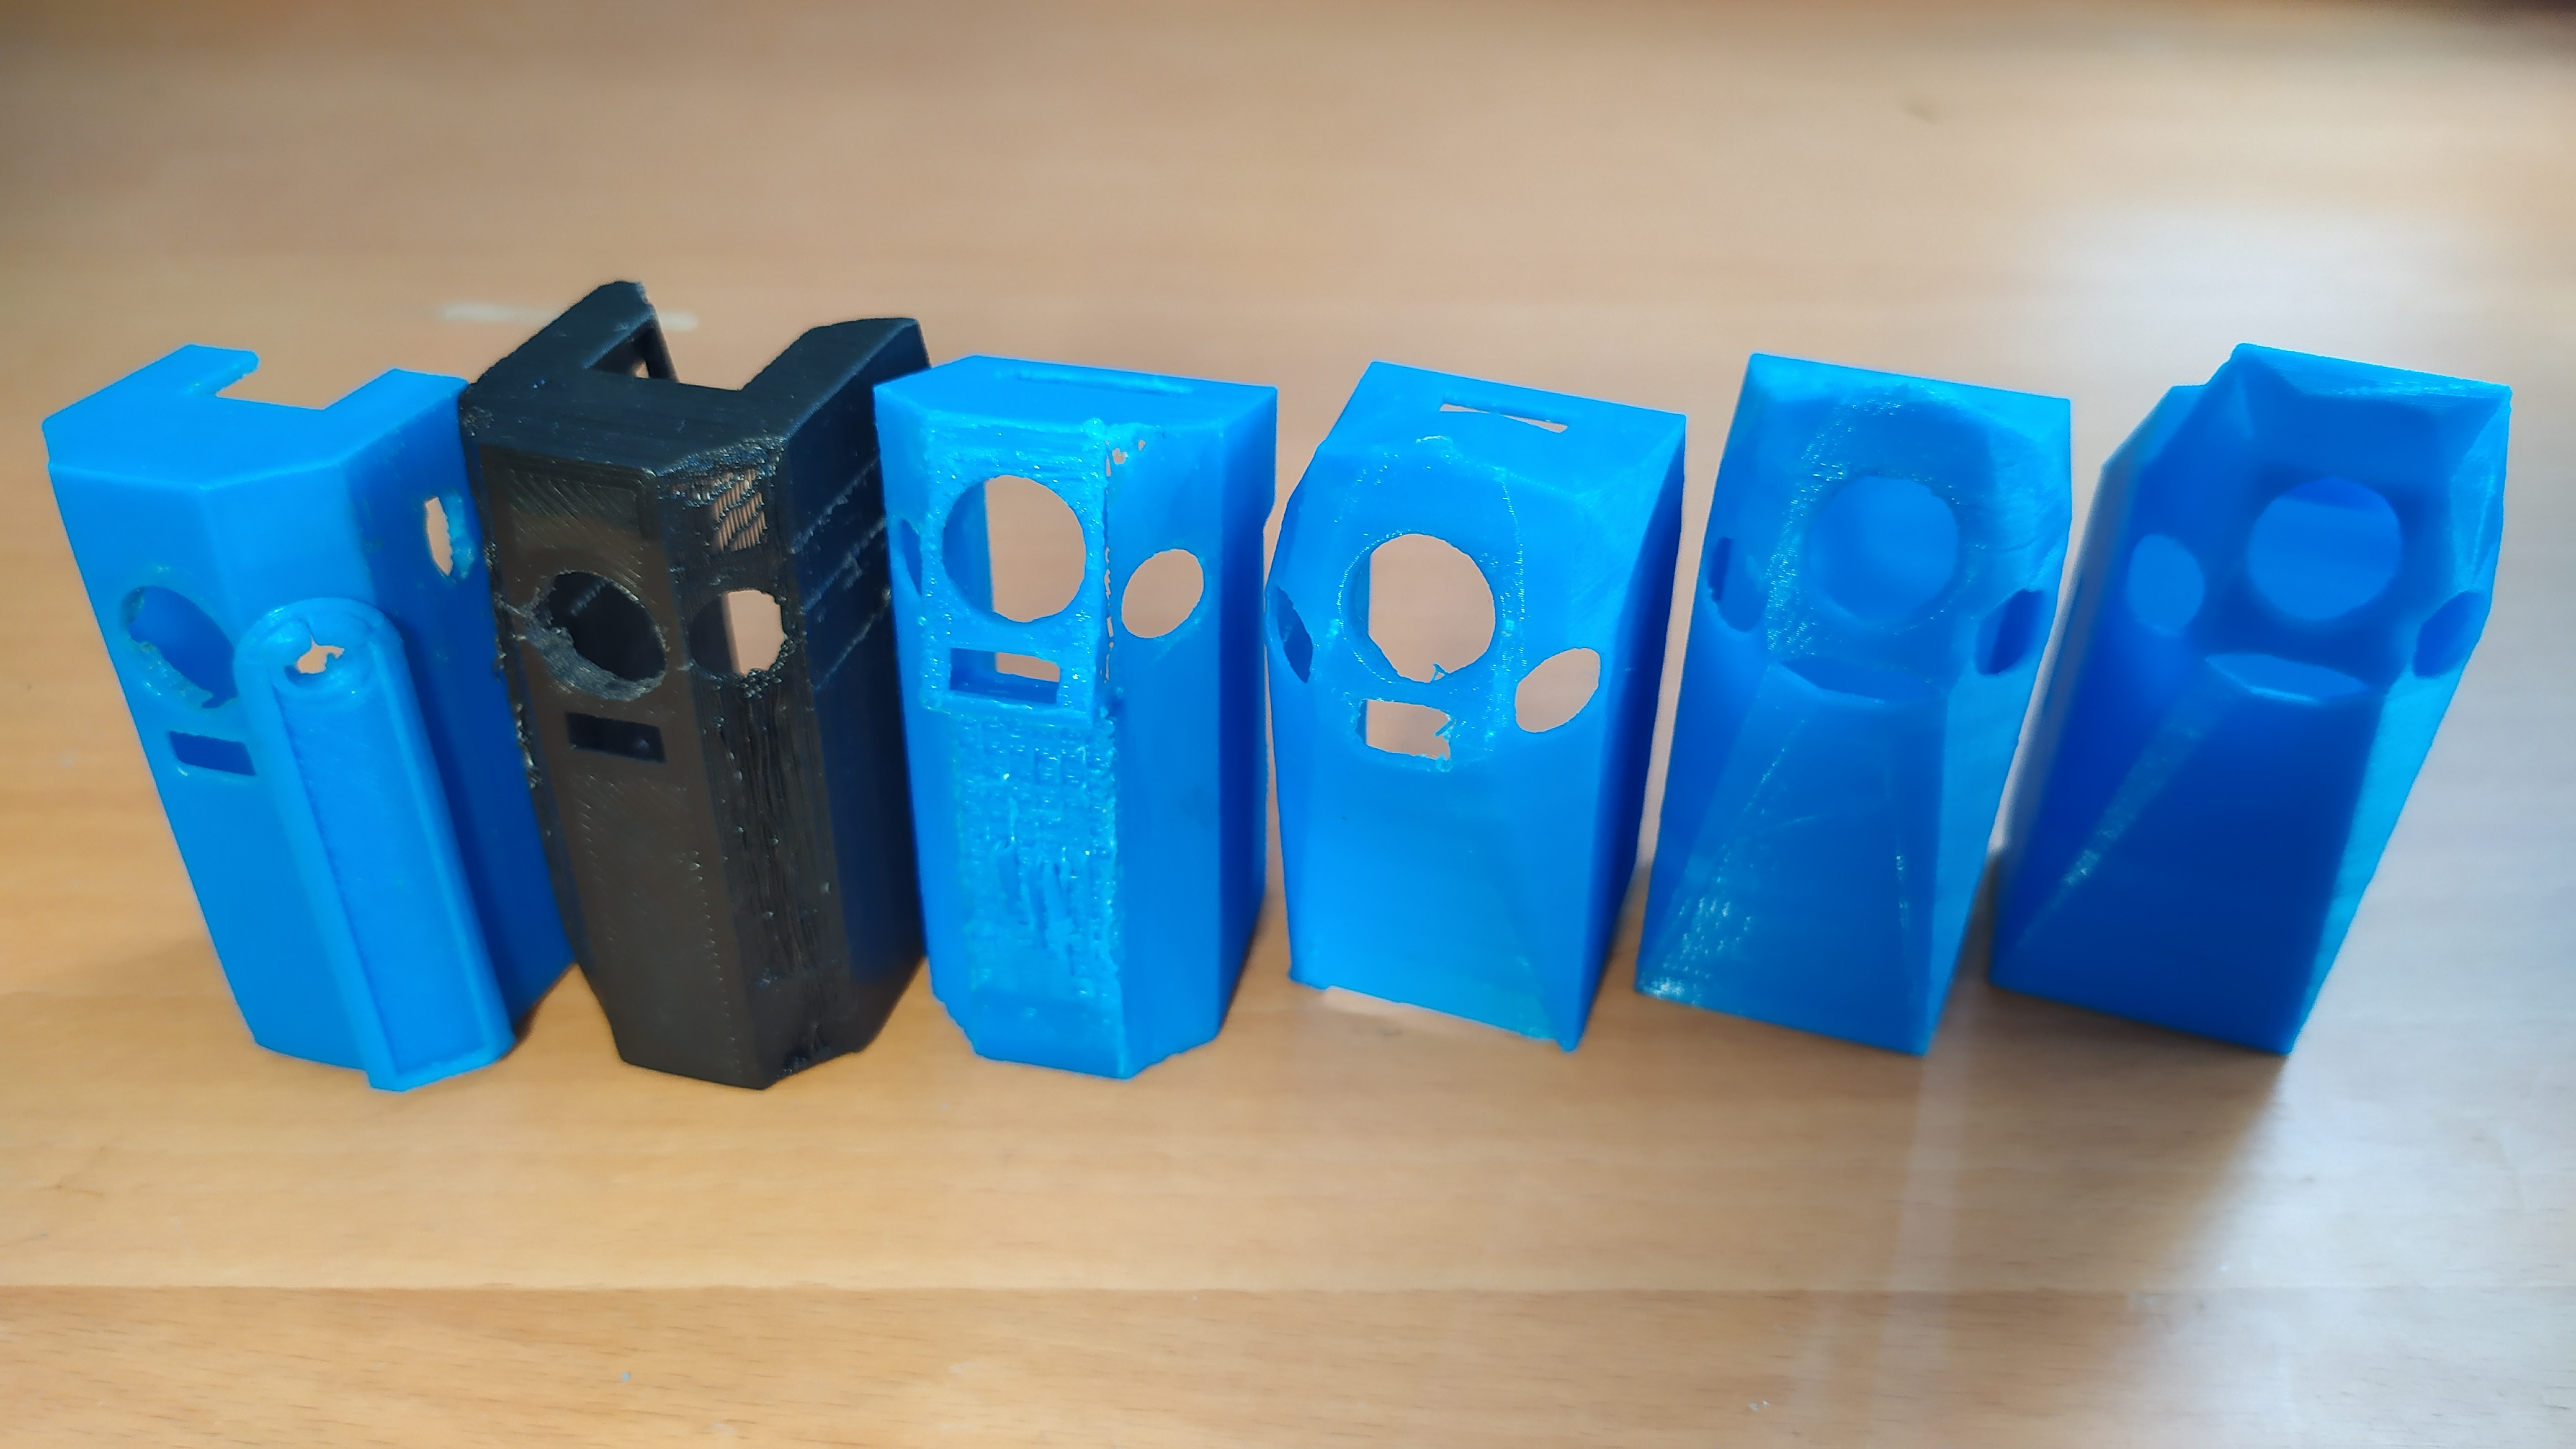
\includegraphics[scale=.1]{imaxes/evolucion-carcasa.jpg}
      \caption{Evolución dos deseños da carcasa.}
      \label{fig:evolucion_carcasa}
    \end{figure}

    \begin{figure}[tbp]
      \centering
      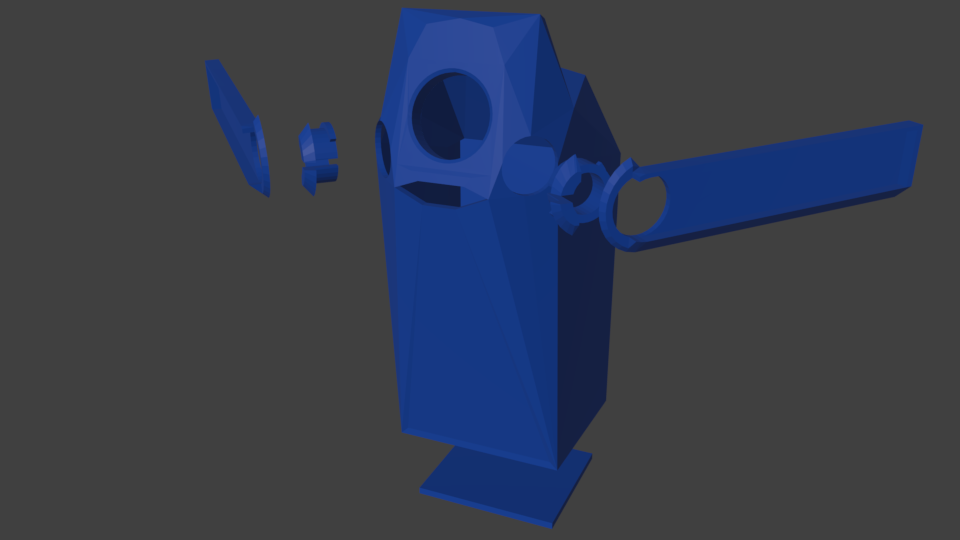
\includegraphics[scale=.4]{imaxes/carcasa.png}
      \caption{Ultimo deseño da carcasa.}
      \label{fig:carcasa}
    \end{figure}
